\documentclass[12pt,a4paper,onecolumn]{exam}
\usepackage{amsmath}
\usepackage{amsthm}
\usepackage{amssymb}
\usepackage{graphicx}
\usepackage{float}
\usepackage{geometry}
\usepackage{tikz}
\usepackage[skins]{tcolorbox}
\usepackage{listings}
\usepackage{xcolor}
\usepackage{hyperref}
\usepackage{multirow}
\usepackage{adjustbox}
\usepackage{booktabs} 
\usepackage[font=small]{caption}
\usepackage{subcaption}

% --- Code Listing Colors ---
\definecolor{codegreen}{rgb}{0,0.6,0}
\definecolor{codegray}{rgb}{0.5,0.5,0.5}
\definecolor{codepurple}{rgb}{0.58,0,0.82}
\definecolor{backcolour}{rgb}{0.95,0.95,0.92}

% --- Code Listing Style ---
\lstdefinestyle{mystyle}{
    backgroundcolor=\color{backcolour},
    commentstyle=\color{codegreen},
    keywordstyle=\color{magenta},
    numberstyle=\tiny\color{codegray},
    stringstyle=\color{codepurple},
    basicstyle=\ttfamily\footnotesize,
    breaklines=true,
    captionpos=b,
    keepspaces=true,
    numbers=left,
    numbersep=2pt,
    showspaces=false,
    showstringspaces=false,
    showtabs=false,
    tabsize=1
}

\newcommand{\questionheader}[1]{%
  \begin{tcolorbox}[
    enhanced,
    colback=black,
    coltext=white,
    boxrule=0pt,
    fontupper=\Large\bfseries,
    arc=4mm
  ]
  #1
  \end{tcolorbox}%
}

\lstset{style=mystyle, language=Python}

\begin{document}

\begingroup
    \centering
    \LARGE E1 213 Pattern Recognition and Neural Network\\
    \LARGE Assignment 1\\[0.5em]
    \large Dwaipayan Haldar\par
    \large \today\\[0.5em]
\endgroup
\noindent\rule{\textwidth}{0.5pt}
\printanswers
\renewcommand{\solutiontitle}{\noindent\textbf{Ans:}\enspace}


\questionheader{Phase 1: Bio-Optic Sensor Calibration}

\textbf{1.1 Gradient Descent vs. Closed Form}
\begin{solution}
Ordinary least squares solution is implemented via the closed form solution $(X^TX)^{-1}Xy$ and also using the vectorized gradient descent algorithm with learning rate $\alpha = 0.01$ and number of iterations equal to 2000. The L2 norm difference between the two methods comes as $1.62 \times 10^{-14}$. 
\end{solution}

\textbf{1.2 Primal to Dual Translation}
\begin{solution}
The target dataset is threshold by median to give a binary dataset. The data is not linearly separable. So hard margin SVM will not be able to fit in the data. I used \verb|scipy.optimize.minimize| to optimize, it is not able to converge and going on some infinite loop. Using \verb|cvxopt.solvers.qp| was able to solve the problem but all the mu was very large suggesting that all of them are support vectors which is clearly not the case. So they are all garbage values.
%What is the optimization technique used in scipy and what is used in cvxopt. Check
\end{solution}

\questionheader{Phase 2: Oncology Array}

\textbf{2.3 The Singularity Trap}
\begin{solution}
Since $D>N$, so the rank of the matrix can be at best $N$ and $X^TX$ is a $1000\times1000$ matrix. So clearly, the matrix is singular. There is no \verb|LinAlgError| in this case because of floating point approximation. But the high condition number of $9.66 \times 10^{18}$ shows that the inverse is unstable and not reliable. Fig. \ref{fig:2_3} gives the condition number vs $\lambda$ values plot, it can be seen with the increase of lambda there is a decrease in the condition number.
\end{solution}

\textbf{2.4 Lasso Sparsity}
\begin{solution}
Fig. \ref{fig:2_4} shows the variation of the $l_1$ norm of weight value with $log(\lambda)$. The exact value of $\lambda$ for which exactly $50\%$ is equal to $0$ is $0.37$. 
\end{solution}

\begin{figure}[H]
\centering
\begin{subfigure}[b]{0.48\textwidth}
    \centering
    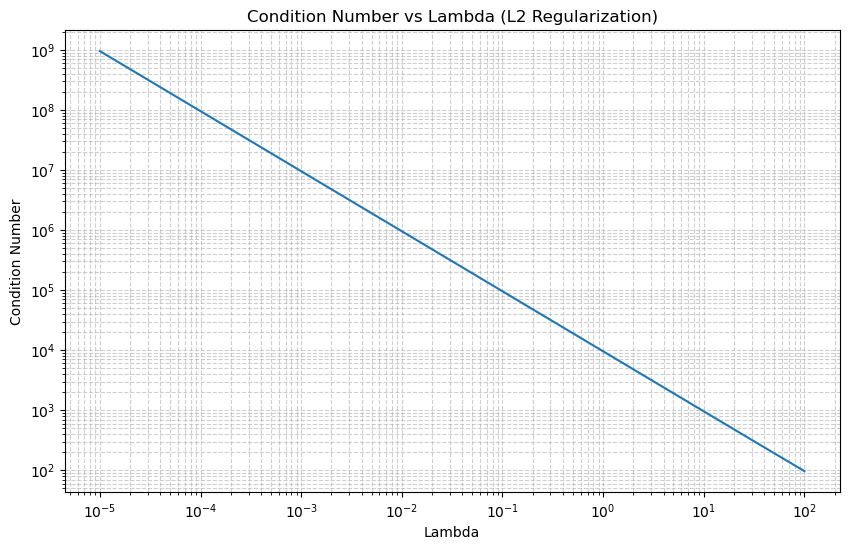
\includegraphics[width=\textwidth]{P02_3.png}
    \caption{$\kappa$ vs $\lambda$ for $l_1$ regularization}
    \label{fig:2_3}
\end{subfigure}
\hfill
\begin{subfigure}[b]{0.48\textwidth}
    \centering
    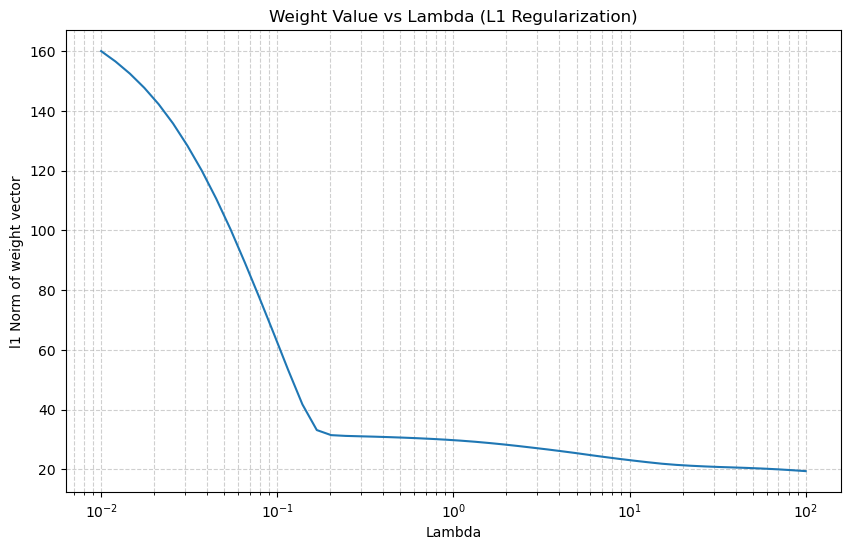
\includegraphics[width=\textwidth]{P02_4.png}
    \caption{$l_1$ norm of the weight vector vs $\log(\lambda)$}
    \label{fig:2_4}
\end{subfigure}
\end{figure}

\questionheader{Phase 3: High Frequency ICU Telemetry}

\textbf{3.5 Vectorized Logistic Regression}
\begin{solution}
The Lipschitz smoothness factor for this case is very small $\frac{1}{L} = 0.003396$. So even when 2 or 3 times the factor is taken, the curve converges as the absolute value of the $\alpha$ is small. Only when very high value is taken then the curve does not converge. Fig. \ref{fig:3_5a} gives the loss curve for a $\alpha$ that is close to the factor and Fig. \ref{fig:3_5b} gives the loss curve for a very high $\alpha$. 
\end{solution}

\begin{figure}[H]
\centering
\begin{subfigure}[b]{0.48\textwidth}
    \centering
    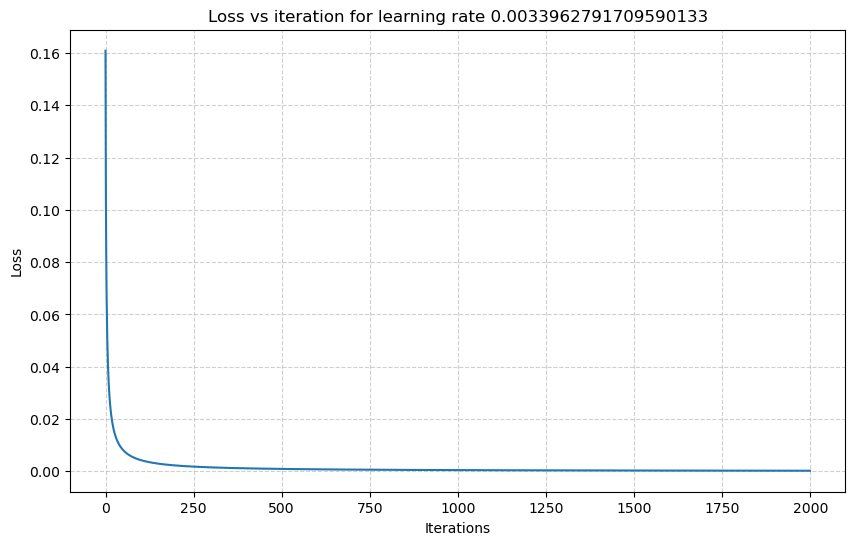
\includegraphics[width=\textwidth]{P03_5a.png}
    \caption{Loss vs iteration curve for $\alpha = 0.00339$}
    \label{fig:3_5a}
\end{subfigure}
\hfill
\begin{subfigure}[b]{0.48\textwidth}
    \centering
    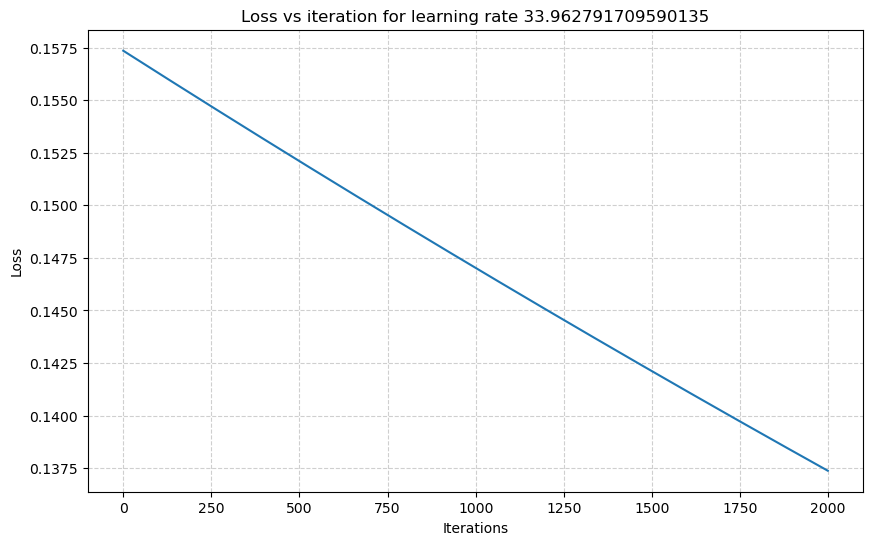
\includegraphics[width=\textwidth]{P03_5b.png}
    \caption{Loss vs iteration curve for $\alpha = 33.96$}
    \label{fig:3_5b}
\end{subfigure}
\end{figure}

\textbf{3.6 GMM Intialization \& The E-Step}
\begin{solution}
The initial log likelihood is -2857267.241 and after one iteration the log likelihood becomes -1771352.38.
\end{solution}

\textbf{3.7 EM Convergence and crashes}
\begin{solution}
Fig. \ref{fig:3_7a}, Fig. \ref{fig:3_7b} and Fig. \ref{fig:3_7c} gives the plots of Log-Likelihood vs Iteration for different values of K = 2,4 and 6. When one of the matrix is made singular, then the function cannot invert the matrix for the multivariate normal equation to work, so it cannot calculate the value of the function at that sample. So, the python breaks with error \verb|LinAlgError|. 
\end{solution}
\begin{figure}[H]
\centering
\begin{subfigure}[b]{0.31\textwidth}
    \centering
    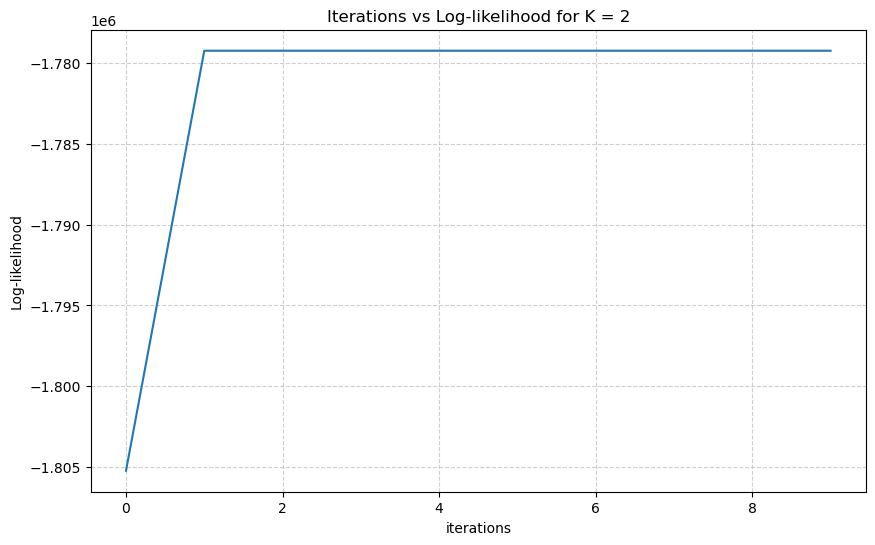
\includegraphics[width=\textwidth]{P03_7a.png}
    \caption{Log-likelihood vs Iteration for $K = 2$}
    \label{fig:3_7a}
\end{subfigure}
\hfill
\begin{subfigure}[b]{0.31\textwidth}
    \centering
    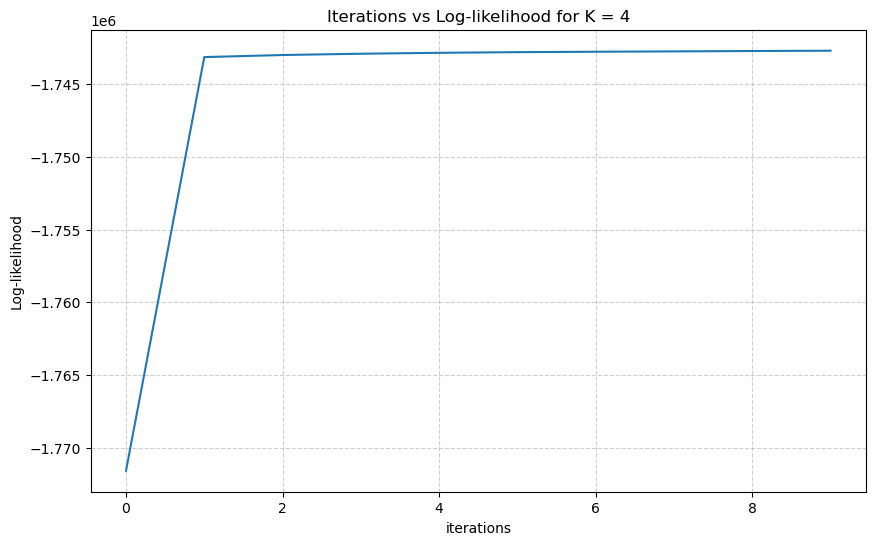
\includegraphics[width=\textwidth]{P03_7b.png}
    \caption{Log-likelihood vs Iteration for $K = 4$}
    \label{fig:3_7b}
\end{subfigure}
\hfill
\begin{subfigure}[b]{0.31\textwidth}
    \centering
    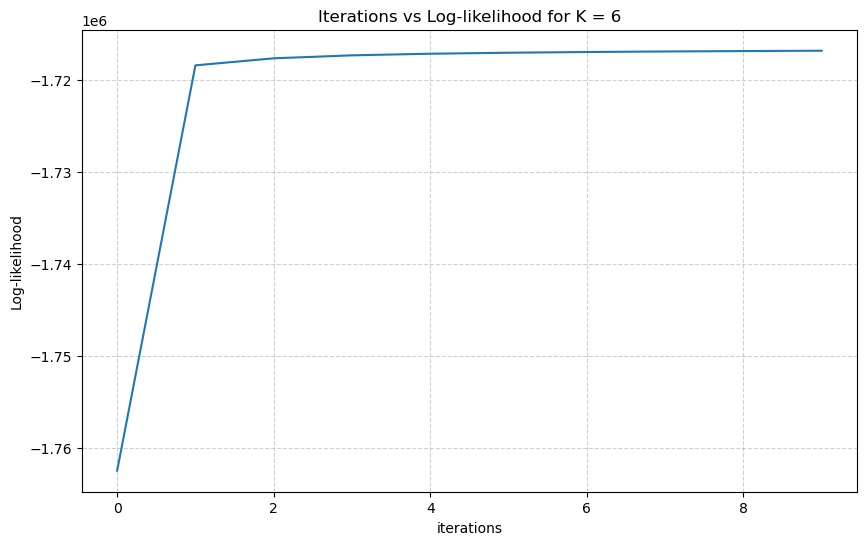
\includegraphics[width=\textwidth]{P03_7c.png}
    \caption{Log-likelihood vs Iteration for $K = 6$}
    \label{fig:3_7c}
\end{subfigure}
\end{figure}

\textbf{3.8 Decision Boundaries}

\begin{solution}
Fig. \ref{fig:3_8} gives the plot of the decision boundary along with the Gaussians.
\end{solution}
\textbf{3.9 SVM with Slack KKT Verification}

\begin{solution}
Index of point exactly on the margin 3374 and the value of mu for this is 0.0004879. Index of point classified safely outside the margin 8564 and the value of mu for this is $7.87 \times 10^{-13}$. No point classified outside the margin, i.e., there is 100\% training accuracy.

\end{solution}
\textbf{3.10 Mercer's Condition}

\begin{solution}
The Kernel matrix satisfy the Mercer's condition. The highest and the lowest eigenvalue is near 1 for small $\lambda$ and when the $\lambda$ becomes high, the matrix is ill conditioned but the lowest eigen value is always greater than 0. 
\end{solution}
\textbf{3.11 Hyperparameter Topography}

\begin{solution}
Fig. \ref{fig:3_11} gives the heatmap of the search in the parameter space. Overfit occurs for all the $C \in \{1,10,100\}$ and $\sigma \in \{0.001,0.01,0.1,1\}$. Only $\sigma = 10$ is able to fit the data properly. 
\end{solution}

\questionheader{Phase 4: Unscaled Electronic Health Records}

\textbf{4.12 Multiclass Extension \& Scaling}
\begin{solution}
The raw data does not converge at all the loss curve oscillates and the loop terminates at 2000 which is the max number of iterations preset. On the other hand, the scaled data converges in 1195 iterations where the tolerance is set to $10^{-6}$.  
\end{solution}

\textbf{4.12 Vectorization Benchmarking}
\begin{solution}
The total time of running the Naive KNN is 25.78 secs, while the vectorized KNN takes only 0.53 secs. That is amost 
\end{solution}

\textbf{4.12 Curse of Scale}
\begin{solution}
The raw data does not converge at all the loss curve oscillates and the loop terminates at 2000 which is the max number of iterations preset. On the other hand, the scaled data converges in 1195 iterations where the tolerance is set to $10^{-6}$.  
\end{solution}


\begin{figure}[H]
\centering
\begin{subfigure}[b]{0.32\textwidth}
    \centering
    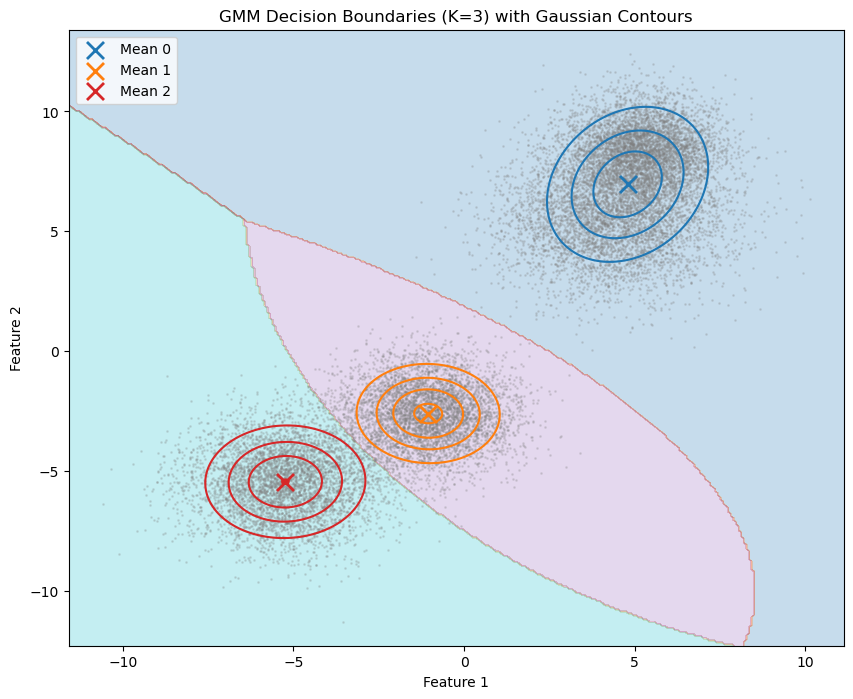
\includegraphics[width=\textwidth]{P03_8.png}
    \caption{GM Decision Boundary}
    \label{fig:3_8}
\end{subfigure}
\hfill
\begin{subfigure}[b]{0.65\textwidth}
    \centering
    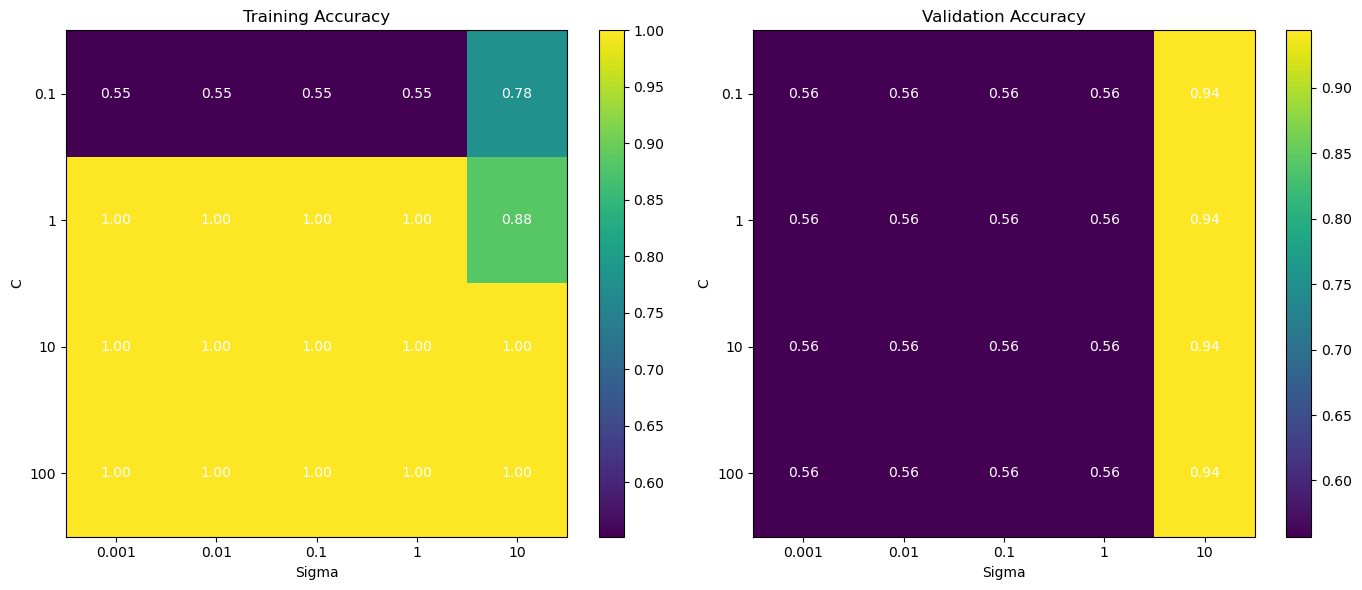
\includegraphics[width=\textwidth]{P03_11.png}
    \caption{Heatmap of the training and validation accuracies}
    \label{fig:3_11}
\end{subfigure}
\end{figure}

\end{document}